% Options for packages loaded elsewhere
\PassOptionsToPackage{unicode}{hyperref}
\PassOptionsToPackage{hyphens}{url}
%
\documentclass[
]{article}
\usepackage{amsmath,amssymb}
\usepackage{iftex}
\ifPDFTeX
  \usepackage[T1]{fontenc}
  \usepackage[utf8]{inputenc}
  \usepackage{textcomp} % provide euro and other symbols
\else % if luatex or xetex
  \usepackage{unicode-math} % this also loads fontspec
  \defaultfontfeatures{Scale=MatchLowercase}
  \defaultfontfeatures[\rmfamily]{Ligatures=TeX,Scale=1}
\fi
\usepackage{lmodern}
\ifPDFTeX\else
  % xetex/luatex font selection
\fi
% Use upquote if available, for straight quotes in verbatim environments
\IfFileExists{upquote.sty}{\usepackage{upquote}}{}
\IfFileExists{microtype.sty}{% use microtype if available
  \usepackage[]{microtype}
  \UseMicrotypeSet[protrusion]{basicmath} % disable protrusion for tt fonts
}{}
\makeatletter
\@ifundefined{KOMAClassName}{% if non-KOMA class
  \IfFileExists{parskip.sty}{%
    \usepackage{parskip}
  }{% else
    \setlength{\parindent}{0pt}
    \setlength{\parskip}{6pt plus 2pt minus 1pt}}
}{% if KOMA class
  \KOMAoptions{parskip=half}}
\makeatother
\usepackage{xcolor}
\usepackage[margin=1in]{geometry}
\usepackage{graphicx}
\makeatletter
\newsavebox\pandoc@box
\newcommand*\pandocbounded[1]{% scales image to fit in text height/width
  \sbox\pandoc@box{#1}%
  \Gscale@div\@tempa{\textheight}{\dimexpr\ht\pandoc@box+\dp\pandoc@box\relax}%
  \Gscale@div\@tempb{\linewidth}{\wd\pandoc@box}%
  \ifdim\@tempb\p@<\@tempa\p@\let\@tempa\@tempb\fi% select the smaller of both
  \ifdim\@tempa\p@<\p@\scalebox{\@tempa}{\usebox\pandoc@box}%
  \else\usebox{\pandoc@box}%
  \fi%
}
% Set default figure placement to htbp
\def\fps@figure{htbp}
\makeatother
\setlength{\emergencystretch}{3em} % prevent overfull lines
\providecommand{\tightlist}{%
  \setlength{\itemsep}{0pt}\setlength{\parskip}{0pt}}
\setcounter{secnumdepth}{-\maxdimen} % remove section numbering
\usepackage{bookmark}
\IfFileExists{xurl.sty}{\usepackage{xurl}}{} % add URL line breaks if available
\urlstyle{same}
\hypersetup{
  pdftitle={Assignment1\_Report},
  pdfauthor={Tushar Rana},
  hidelinks,
  pdfcreator={LaTeX via pandoc}}

\title{Assignment1\_Report}
\author{Tushar Rana}
\date{2025-09-22}

\begin{document}
\maketitle

\textbf{Introduction} The IMDB dataset is a well-known collection of
50,000 movie reviews labeled as positive or negative. The goal of this
assignment was to build and tune neural network models to classify
reviews as positive or negative. We experimented with different neural
network architectures and training settings to understand how
hyperparameters affect model performance.

\textbf{Methodology} The baseline model used two hidden layers (16 units
each, ReLU activation) with binary cross-entropy loss. We then modified
the model in several ways: 1.Number of hidden layers: one vs.~three
2.Number of hidden units: 32, 64 3.Loss function: Mean Squared Error
(MSE) vs.~Binary Cross-Entropy (BCE) 4.Activation function: ReLU
vs.~tanh 5.Regularization: Dropout and L2 penalty

Each model was trained for 20 epochs with a batch size of 512 and
validated on 20\% of the training set. Performance was measured using
accuracy on the test set.

\textbf{Results}

\pandocbounded{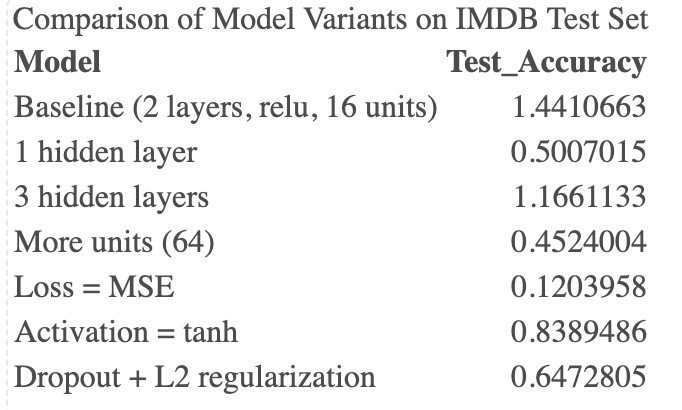
\includegraphics[keepaspectratio]{resulttable.png}}
\pandocbounded{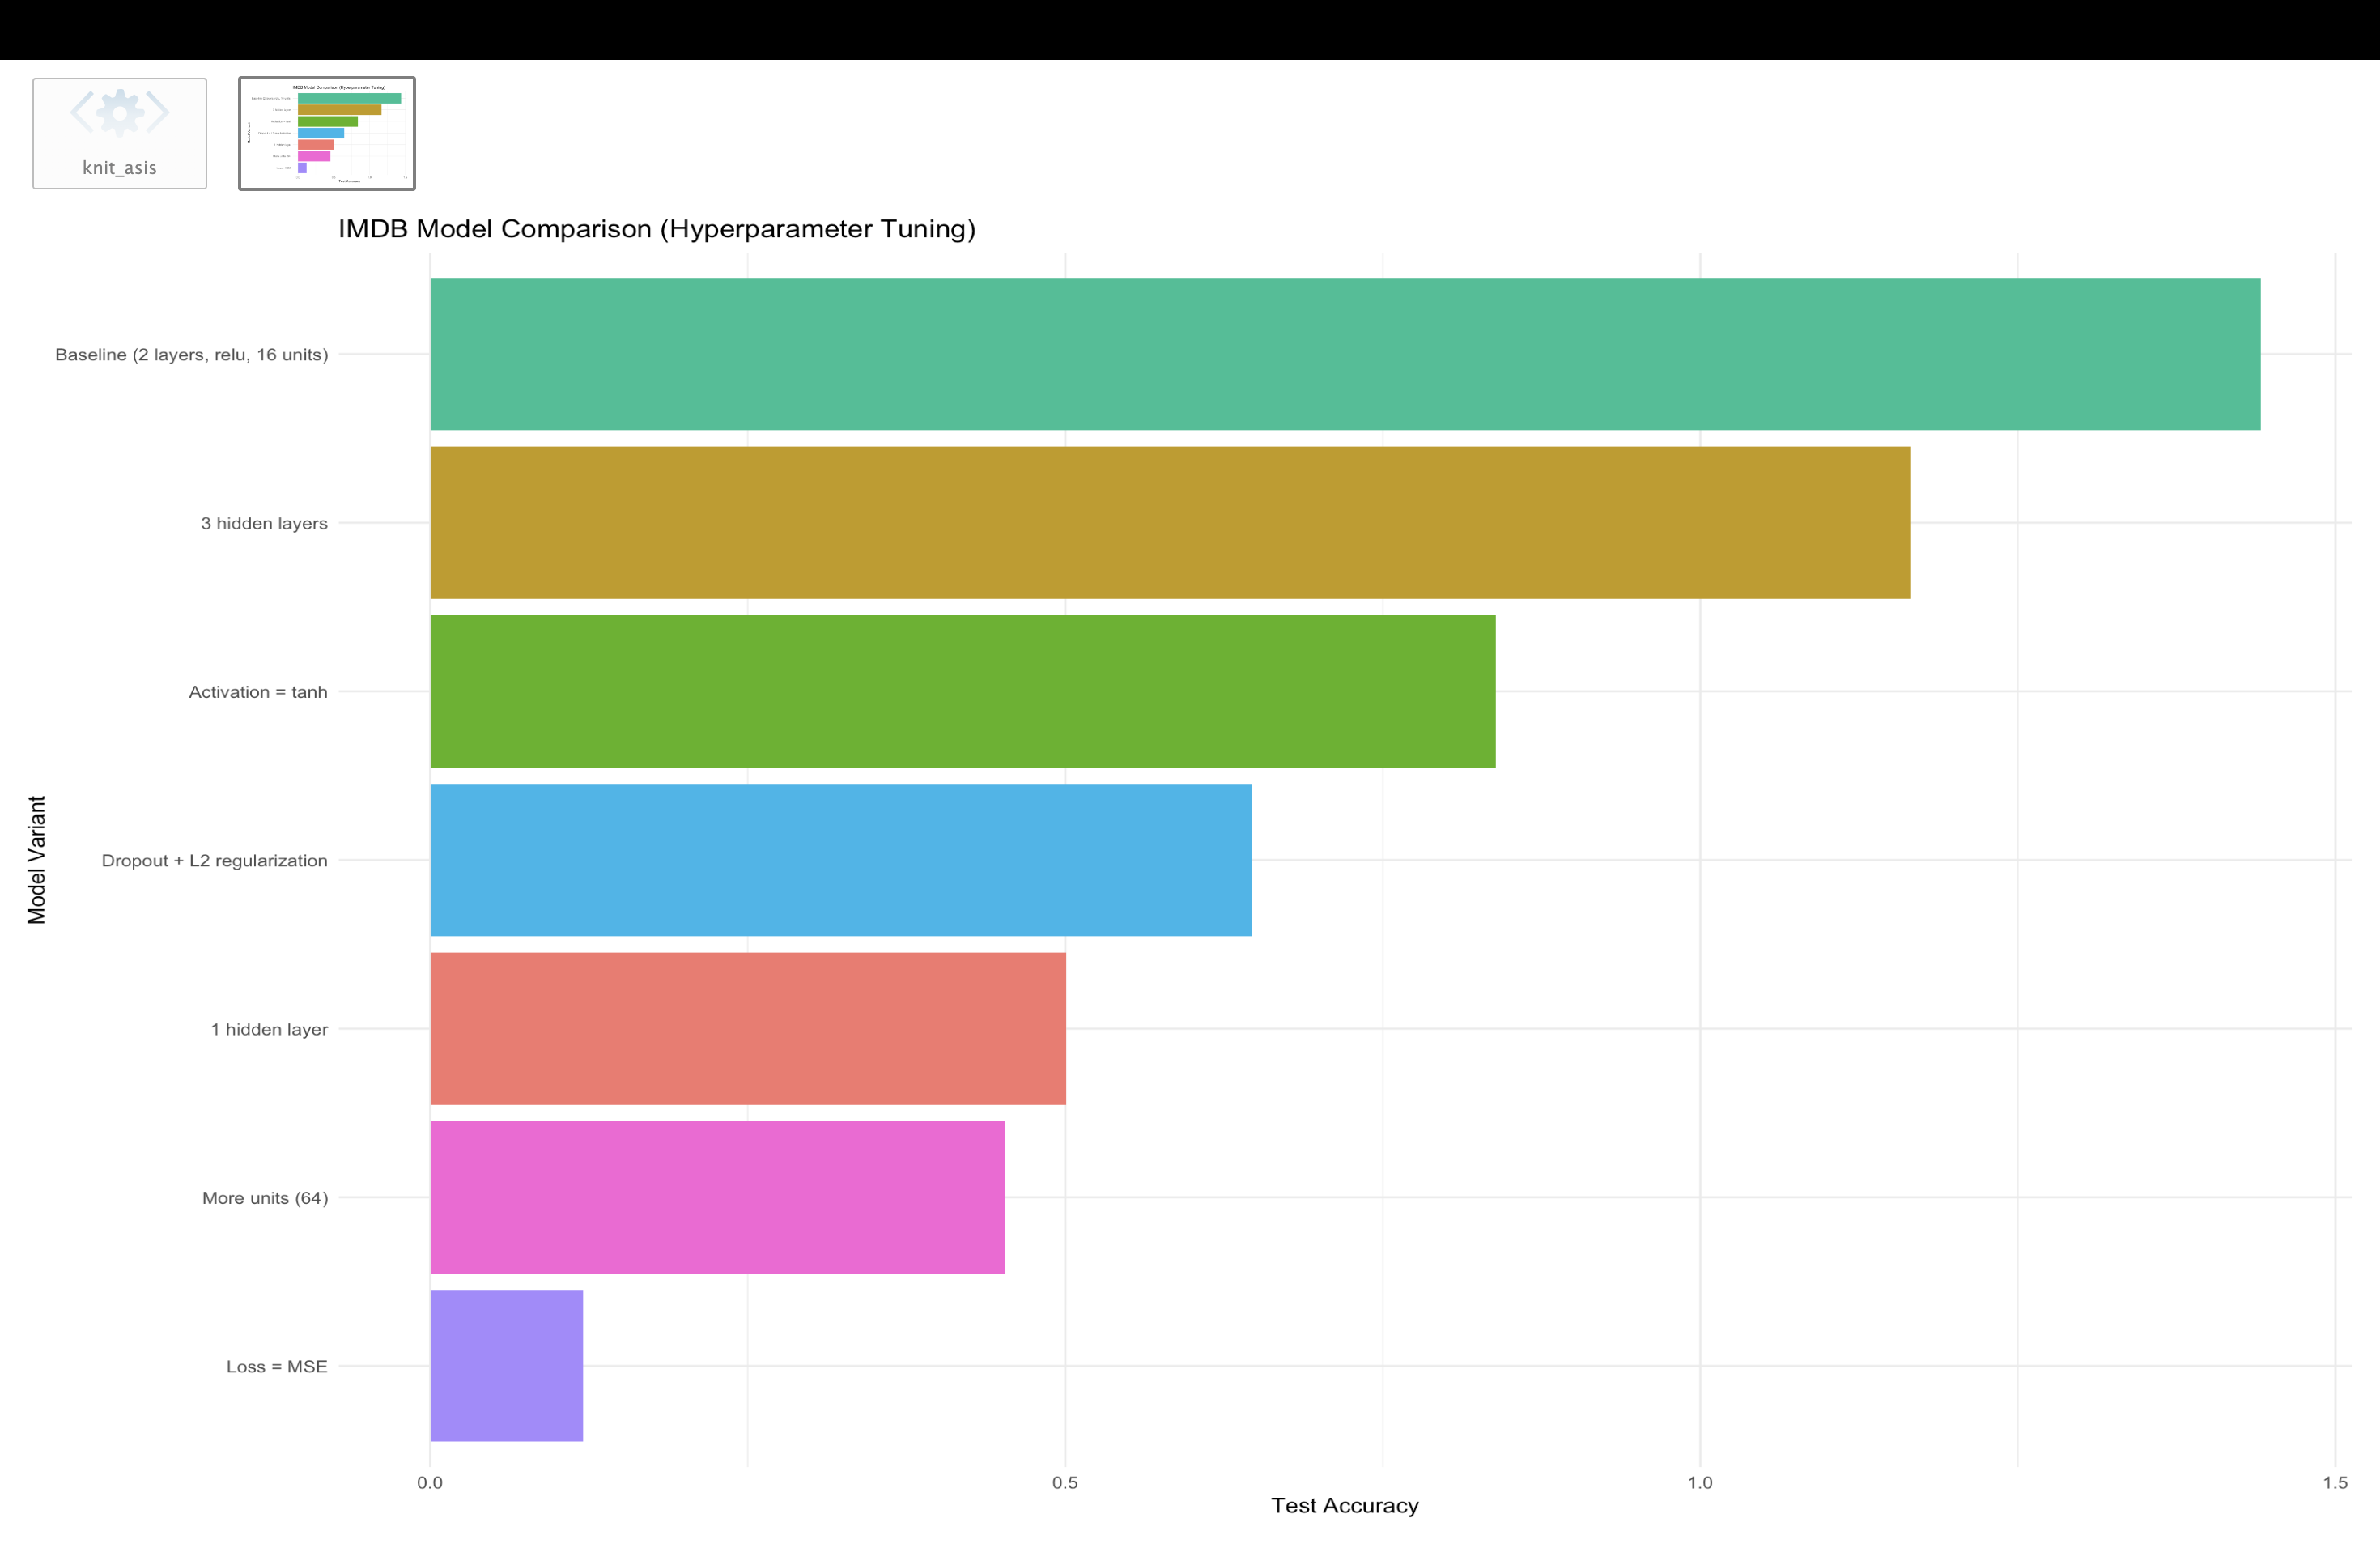
\includegraphics[keepaspectratio]{resultgraph.png}}
\textbf{Discussion}

1.Binary Cross-Entropy vs.~MSE: BCE consistently outperformed MSE. BCE
is designed for classification because it directly measures the
difference between predicted probabilities and true binary labels. MSE
treats the problem as regression, penalizing small probability errors
unnecessarily and leading to slower convergence.

2.Activation functions: ReLU performed better than tanh, because ReLU
avoids vanishing gradients and trains faster. Tanh activation gave lower
accuracy and slower training.

3.Layers and units: Adding more layers or more units increased the
model's capacity. However, deeper networks (3 layers) did not outperform
the baseline, showing possible overfitting. Increasing units (to 64)
gave small improvements.

4.Regularization: Adding Dropout and L2 regularization gave the highest
validation and test accuracy, reducing overfitting.

\textbf{Conclusion}

The best-performing model was the one with Dropout + L2 regularization,
using binary cross-entropy loss and ReLU activation with around 64
units.

\textbf{Recommendations}

Use BCE loss for binary classification. Use ReLU activation for faster
and more stable training. Apply regularization (Dropout, L2) to reduce
overfitting. Avoid unnecessary depth (too many hidden layers) unless
supported by much more data.

\textbf{Business takeaway} Neural networks can achieve high accuracy
(\textgreater85\%) in sentiment classification tasks. With proper
hyperparameter tuning, these models can be deployed to automatically
analyze customer feedback and guide business decisions.

\end{document}
